\documentclass{standalone}
\usepackage{tikz}
\usetikzlibrary{patterns, positioning}

\begin{document}
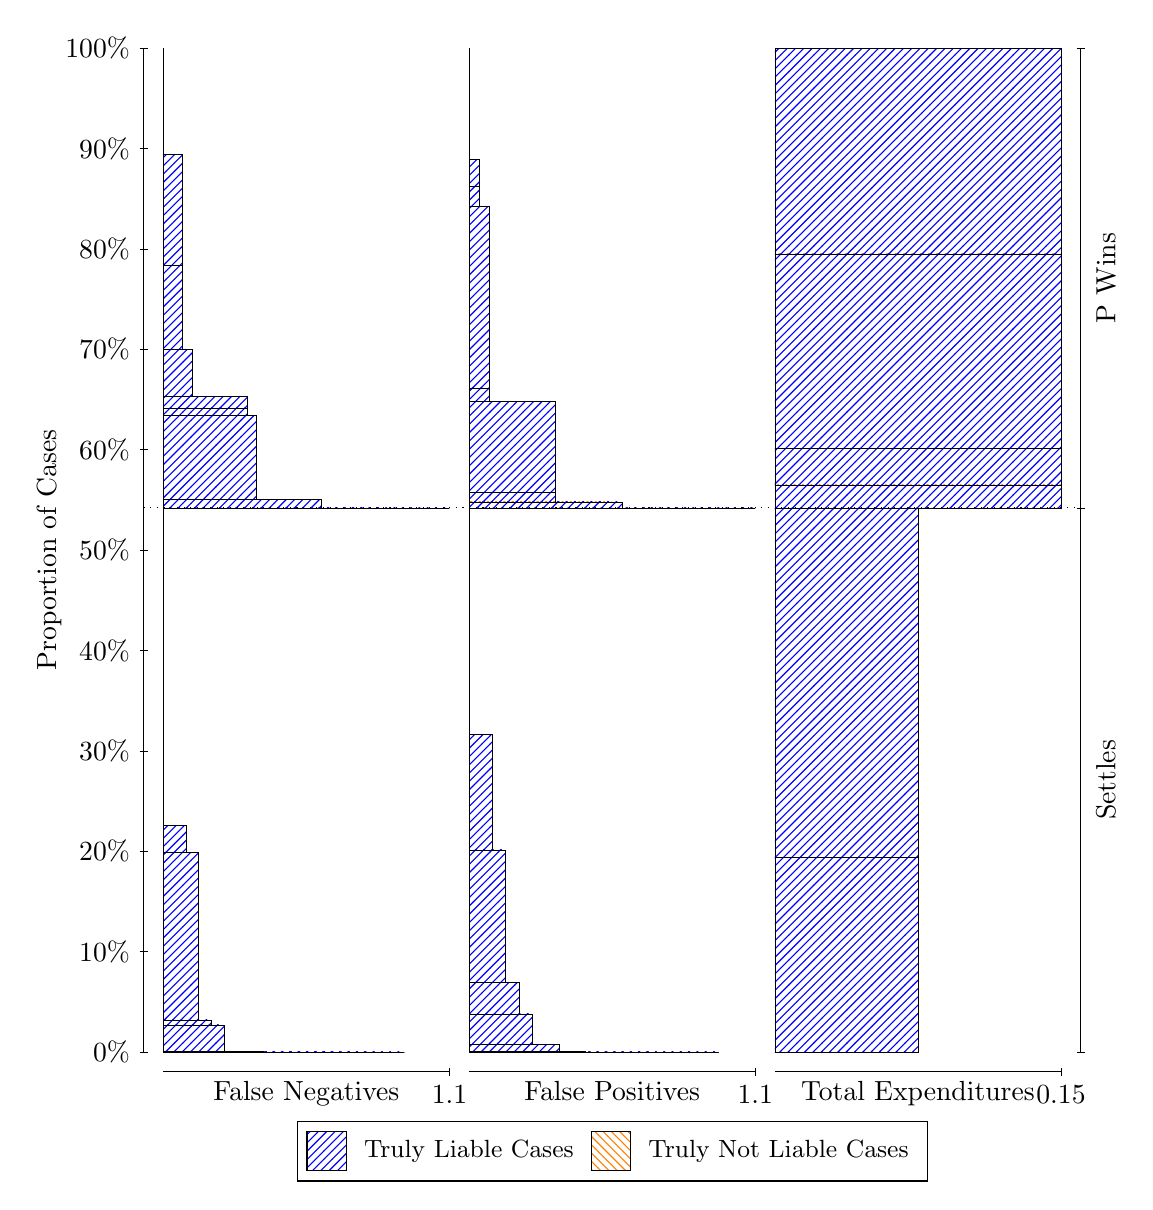
\begin{tikzpicture}
\draw[black, very thin] (1.5,1.75) -- (1.5,14.5);
\node[rotate=90, anchor=center] at (0.3, 8.125) {Proportion of Cases};
\draw[black, very thin] (1.45,1.75) -- (1.55,1.75);
\node[anchor=east] at (1.45, 1.75) {0\%};
\draw[black, very thin] (1.45,3.025) -- (1.55,3.025);
\node[anchor=east] at (1.45, 3.025) {10\%};
\draw[black, very thin] (1.45,4.3) -- (1.55,4.3);
\node[anchor=east] at (1.45, 4.3) {20\%};
\draw[black, very thin] (1.45,5.575) -- (1.55,5.575);
\node[anchor=east] at (1.45, 5.575) {30\%};
\draw[black, very thin] (1.45,6.85) -- (1.55,6.85);
\node[anchor=east] at (1.45, 6.85) {40\%};
\draw[black, very thin] (1.45,8.125) -- (1.55,8.125);
\node[anchor=east] at (1.45, 8.125) {50\%};
\draw[black, very thin] (1.45,9.4) -- (1.55,9.4);
\node[anchor=east] at (1.45, 9.4) {60\%};
\draw[black, very thin] (1.45,10.675) -- (1.55,10.675);
\node[anchor=east] at (1.45, 10.675) {70\%};
\draw[black, very thin] (1.45,11.95) -- (1.55,11.95);
\node[anchor=east] at (1.45, 11.95) {80\%};
\draw[black, very thin] (1.45,13.225) -- (1.55,13.225);
\node[anchor=east] at (1.45, 13.225) {90\%};
\draw[black, very thin] (1.45,14.5) -- (1.55,14.5);
\node[anchor=east] at (1.45, 14.5) {100\%};

\draw[black, very thin] (13.4,1.75) -- (13.4,14.5);
\draw[black, very thin] (13.35,1.75) -- (13.45,1.75);
\node[anchor=west] at (13.35, 1.75) {};
\draw[black, very thin] (13.35,8.66) -- (13.45,8.66);
\node[anchor=west] at (13.35, 8.66) {};
\draw[black, very thin] (13.35,14.5) -- (13.45,14.5);
\node[anchor=west] at (13.35, 14.5) {};

\draw[black, very thin, pattern color=blue, pattern=north east lines] (1.75,1.75) rectangle (4.8118,1.75);
\draw[black, very thin, pattern color=blue, pattern=north east lines] (1.75,1.75) rectangle (4.4852,1.75);
\draw[black, very thin, pattern color=blue, pattern=north east lines] (1.75,1.75) rectangle (4.1586,1.75);
\draw[black, very thin, pattern color=blue, pattern=north east lines] (1.75,1.75) rectangle (3.9953,1.75);
\draw[black, very thin, pattern color=blue, pattern=north east lines] (1.75,1.75) rectangle (3.832,1.75);
\draw[black, very thin, pattern color=blue, pattern=north east lines] (1.75,1.75) rectangle (3.6687,1.75);
\draw[black, very thin, pattern color=blue, pattern=north east lines] (1.75,1.75) rectangle (3.5054,1.75);
\draw[black, very thin, pattern color=blue, pattern=north east lines] (1.75,1.75) rectangle (3.3421,1.7505);
\draw[black, very thin, pattern color=blue, pattern=north east lines] (1.75,1.7505) rectangle (3.1788,1.7506);
\draw[black, very thin, pattern color=blue, pattern=north east lines] (1.75,1.7506) rectangle (3.0155,1.7529);
\draw[black, very thin, pattern color=blue, pattern=north east lines] (1.75,1.7529) rectangle (2.8522,1.7558);
\draw[black, very thin, pattern color=blue, pattern=north east lines] (1.75,1.7558) rectangle (2.689,1.7558);
\draw[black, very thin, pattern color=blue, pattern=north east lines] (1.75,1.7558) rectangle (2.5257,2.0933);
\draw[black, very thin, pattern color=blue, pattern=north east lines] (1.75,2.0933) rectangle (2.3624,2.1571);
\draw[black, very thin, pattern color=blue, pattern=north east lines] (1.75,2.1571) rectangle (2.1991,4.2893);
\draw[black, very thin, pattern color=blue, pattern=north east lines] (1.75,4.2893) rectangle (2.0358,4.6271);
\draw[black, very thin, pattern color=blue, pattern=north east lines] (1.75,4.6271) rectangle (1.8725,4.6272);
\draw[black, very thin, pattern color=orange, pattern=north west lines] (1.75,4.6272) rectangle (1.75,4.6272);
\draw[black, very thin, pattern color=blue, pattern=north east lines] (1.75,4.6272) rectangle (1.75,8.66);
\draw[black, very thin, pattern color=blue, pattern=north east lines] (1.75,8.66) rectangle (5.3833,8.66);
\draw[black, very thin, pattern color=blue, pattern=north east lines] (1.75,8.66) rectangle (4.5669,8.6612);
\draw[black, very thin, pattern color=blue, pattern=north east lines] (1.75,8.6612) rectangle (4.4444,8.6612);
\draw[black, very thin, pattern color=blue, pattern=north east lines] (1.75,8.6612) rectangle (3.7504,8.7723);
\draw[black, very thin, pattern color=blue, pattern=north east lines] (1.75,8.7723) rectangle (3.6279,8.7724);
\draw[black, very thin, pattern color=blue, pattern=north east lines] (1.75,8.7724) rectangle (2.9339,9.8335);
\draw[black, very thin, pattern color=blue, pattern=north east lines] (1.75,9.8335) rectangle (2.8114,9.9294);
\draw[black, very thin, pattern color=blue, pattern=north east lines] (1.75,9.9294) rectangle (2.8114,10.077);
\draw[black, very thin, pattern color=blue, pattern=north east lines] (1.75,10.077) rectangle (2.1174,10.676);
\draw[black, very thin, pattern color=blue, pattern=north east lines] (1.75,10.676) rectangle (1.9949,11.742);
\draw[black, very thin, pattern color=blue, pattern=north east lines] (1.75,11.742) rectangle (1.9949,13.147);
\draw[black, very thin, pattern color=orange, pattern=north west lines] (1.75,13.147) rectangle (1.75,13.147);
\draw[black, very thin, pattern color=blue, pattern=north east lines] (1.75,13.147) rectangle (1.75,14.5);
\draw[black, very thin, pattern color=orange, pattern=north west lines] (5.6333,1.75) rectangle (8.8019,1.75);
\draw[black, very thin, pattern color=blue, pattern=north east lines] (5.6333,1.75) rectangle (8.8019,1.75);
\draw[black, very thin, pattern color=blue, pattern=north east lines] (5.6333,1.75) rectangle (7.957,1.75);
\draw[black, very thin, pattern color=orange, pattern=north west lines] (5.6333,1.75) rectangle (7.788,1.75);
\draw[black, very thin, pattern color=blue, pattern=north east lines] (5.6333,1.75) rectangle (7.788,1.75);
\draw[black, very thin, pattern color=orange, pattern=north west lines] (5.6333,1.75) rectangle (7.45,1.75);
\draw[black, very thin, pattern color=blue, pattern=north east lines] (5.6333,1.75) rectangle (7.45,1.75);
\draw[black, very thin, pattern color=orange, pattern=north west lines] (5.6333,1.75) rectangle (7.112,1.75);
\draw[black, very thin, pattern color=blue, pattern=north east lines] (5.6333,1.75) rectangle (7.112,1.7529);
\draw[black, very thin, pattern color=blue, pattern=north east lines] (5.6333,1.7529) rectangle (6.943,1.7529);
\draw[black, very thin, pattern color=orange, pattern=north west lines] (5.6333,1.7529) rectangle (6.774,1.7529);
\draw[black, very thin, pattern color=blue, pattern=north east lines] (5.6333,1.7529) rectangle (6.774,1.8428);
\draw[black, very thin, pattern color=blue, pattern=north east lines] (5.6333,1.8428) rectangle (6.605,1.8428);
\draw[black, very thin, pattern color=orange, pattern=north west lines] (5.6333,1.8428) rectangle (6.436,1.8428);
\draw[black, very thin, pattern color=blue, pattern=north east lines] (5.6333,1.8428) rectangle (6.436,2.233);
\draw[black, very thin, pattern color=blue, pattern=north east lines] (5.6333,2.233) rectangle (6.2671,2.6365);
\draw[black, very thin, pattern color=orange, pattern=north west lines] (5.6333,2.6365) rectangle (6.0981,2.6365);
\draw[black, very thin, pattern color=blue, pattern=north east lines] (5.6333,2.6365) rectangle (6.0981,4.3155);
\draw[black, very thin, pattern color=blue, pattern=north east lines] (5.6333,4.3155) rectangle (6.0981,4.316);
\draw[black, very thin, pattern color=blue, pattern=north east lines] (5.6333,4.316) rectangle (5.9291,5.7828);
\draw[black, very thin, pattern color=blue, pattern=north east lines] (5.6333,5.7828) rectangle (5.7601,5.7828);
\draw[black, very thin, pattern color=blue, pattern=north east lines] (5.6333,5.7828) rectangle (5.6333,8.66);
\draw[black, very thin, pattern color=orange, pattern=north west lines] (5.6333,8.66) rectangle (9.2667,8.66);
\draw[black, very thin, pattern color=blue, pattern=north east lines] (5.6333,8.66) rectangle (9.2667,8.66);
\draw[black, very thin, pattern color=orange, pattern=north west lines] (5.6333,8.66) rectangle (8.4217,8.66);
\draw[black, very thin, pattern color=blue, pattern=north east lines] (5.6333,8.66) rectangle (8.4217,8.6605);
\draw[black, very thin, pattern color=orange, pattern=north west lines] (5.6333,8.6605) rectangle (7.5767,8.6605);
\draw[black, very thin, pattern color=blue, pattern=north east lines] (5.6333,8.6605) rectangle (7.5767,8.7356);
\draw[black, very thin, pattern color=orange, pattern=north west lines] (5.6333,8.7356) rectangle (7.45,8.7356);
\draw[black, very thin, pattern color=blue, pattern=north east lines] (5.6333,8.7356) rectangle (7.45,8.7356);
\draw[black, very thin, pattern color=orange, pattern=north west lines] (5.6333,8.7356) rectangle (6.7318,8.7356);
\draw[black, very thin, pattern color=blue, pattern=north east lines] (5.6333,8.7356) rectangle (6.7318,8.8555);
\draw[black, very thin, pattern color=blue, pattern=north east lines] (5.6333,8.8555) rectangle (6.7318,10.012);
\draw[black, very thin, pattern color=orange, pattern=north west lines] (5.6333,10.012) rectangle (6.605,10.012);
\draw[black, very thin, pattern color=blue, pattern=north east lines] (5.6333,10.012) rectangle (6.605,10.013);
\draw[black, very thin, pattern color=blue, pattern=north east lines] (5.6333,10.013) rectangle (5.8868,10.184);
\draw[black, very thin, pattern color=blue, pattern=north east lines] (5.6333,10.184) rectangle (5.8868,12.484);
\draw[black, very thin, pattern color=orange, pattern=north west lines] (5.6333,12.484) rectangle (5.7601,12.484);
\draw[black, very thin, pattern color=blue, pattern=north east lines] (5.6333,12.484) rectangle (5.7601,12.743);
\draw[black, very thin, pattern color=blue, pattern=north east lines] (5.6333,12.743) rectangle (5.7601,13.083);
\draw[black, very thin, pattern color=blue, pattern=north east lines] (5.6333,13.083) rectangle (5.6333,14.5);
\draw[black, very thin, pattern color=orange, pattern=north west lines] (9.5167,1.75) rectangle (11.333,1.75);
\draw[black, very thin, pattern color=blue, pattern=north east lines] (9.5167,1.75) rectangle (11.333,4.2232);
\draw[black, very thin, pattern color=orange, pattern=north west lines] (9.5167,4.2232) rectangle (11.333,4.2232);
\draw[black, very thin, pattern color=blue, pattern=north east lines] (9.5167,4.2232) rectangle (11.333,8.66);
\draw[black, very thin, pattern color=orange, pattern=north west lines] (9.5167,8.66) rectangle (13.15,8.66);
\draw[black, very thin, pattern color=blue, pattern=north east lines] (9.5167,8.66) rectangle (13.15,8.9521);
\draw[black, very thin, pattern color=orange, pattern=north west lines] (9.5167,8.9521) rectangle (13.15,8.9521);
\draw[black, very thin, pattern color=blue, pattern=north east lines] (9.5167,8.9521) rectangle (13.15,9.4196);
\draw[black, very thin, pattern color=orange, pattern=north west lines] (9.5167,9.4196) rectangle (13.15,9.4196);
\draw[black, very thin, pattern color=blue, pattern=north east lines] (9.5167,9.4196) rectangle (13.15,11.886);
\draw[black, very thin, pattern color=orange, pattern=north west lines] (9.5167,11.886) rectangle (13.15,11.886);
\draw[black, very thin, pattern color=blue, pattern=north east lines] (9.5167,11.886) rectangle (13.15,14.5);
\draw[black, dotted] (1.5,8.66) -- (13.4,8.66);
\draw[black, very thin] (1.75,1.5) -- (5.3833,1.5);
\node[anchor=north] at (3.5667, 1.5) {False Negatives};
\draw[black, very thin] (5.3833,1.45) -- (5.3833,1.55);
\node[anchor=north] at (5.3833, 1.45) {1.1};

\draw[black, very thin] (5.6333,1.5) -- (9.2667,1.5);
\node[anchor=north] at (7.45, 1.5) {False Positives};
\draw[black, very thin] (9.2667,1.45) -- (9.2667,1.55);
\node[anchor=north] at (9.2667, 1.45) {1.1};

\draw[black, very thin] (9.5167,1.5) -- (13.15,1.5);
\node[anchor=north] at (11.333, 1.5) {Total Expenditures};
\draw[black, very thin] (13.15,1.45) -- (13.15,1.55);
\node[anchor=north] at (13.15, 1.45) {0.15};

\node[black, centered, rotate=90] at (13.72, 5.205) {Settles};
\node[black, centered, rotate=90] at (13.72, 11.58) {P Wins};

\draw (7.449999999999999,1.5) node[draw=none] (baseCoordinate) {};
\begin{scope}[align=center]
        \matrix[scale=0.5, draw=black, below=0.5cm of baseCoordinate, nodes={draw}, column sep=0.1cm]{
            \node[rectangle, draw, minimum width=0.5cm, minimum height=0.5cm, pattern=north east lines, pattern color=blue] {}; &
            \node[draw=none, font=\small] (B) {Truly Liable Cases}; &
            \node[rectangle, draw, minimum width=0.5cm, minimum height=0.5cm, pattern=north west lines, pattern color=orange] {}; &
            \node[draw=none, font=\small] (B) {Truly Not Liable Cases}; \\
            };
\end{scope}

\end{tikzpicture}
\end{document}